
\chapter{Requirements and tools}

The project requirements outline the system's expected functions and performance, detailing the features and capabilities that meet user needs. This forms the foundation for designing and implementing the system's core functionalities.

\section{Functional Requirements}

Functional requirements define the specific behavior and functions of the system. For the dice game application, these include:
\begin{enumerate}
\item {\bfseries AI Opponent}: The system should feature an AI opponent that dynamically adapts to player behavior and skill level.
\item {\bfseries Game Variants}: The application should support a variety of dice games, providing diverse gameplay options.
\item {\bfseries Player Analytics}: The system should track and analyze player statistics to inform AI decision-making.
\item {\bfseries User Interface}: The application should provide an intuitive and consistent user interface for all game variants.
\item {\bfseries Real-Time Feedback}: Users should receive performance feedback, to understand and improve their gameplay strategies.
\item {\bfseries Image Recognition}: The system should accurately detect and recognize physical dice through the device camera:
    \begin{itemize}
        \item Detect dice faces in real-time using computer vision
        \item Process multiple dice simultaneously
        \item Provide accurate pip counting and value recognition
    \end{itemize}
\end{enumerate}
\section{Non-functional Requirements}
Non-functional requirements are essential for ensuring the quality and performance of the system. They help address issues such as latency, scalability, usability, reliability, and security. For the application, the following non-functional requirements are identified:
\begin{enumerate}
\item {\bfseries Performance}: The application should deliver a smooth user experience on mobile devices, with minimal latency in AI decision-making.
\item {\bfseries Scalability}: The system should be able to handle an increasing number of users and game variants.
\item {\bfseries Usability}: The user interface should be easy to navigate and accessible to diverse users.
\item {\bfseries Reliability}: The application should consistently provide accurate AI behavior and player analytics, maintaining user satisfaction.
\end{enumerate}

\section{Use Case Modelling}
Use cases describe how users interact with the system, illustrated using UML diagrams that visualize user interactions and the application's features.

\begin{figure}[h]
    \centering
    \includesvg[scale=0.9]{uml/render/main_menu_usecase.svg}
    \caption{Use case for the game's main menu.}
    \label{fig:main_menu_usecase}
\end{figure}

\begin{figure}[h]
    \centering
    \includesvg[scale=0.7]{uml/render/game_usecase.svg}
    \caption{Use case for the game's core gameplay.}
    \label{fig:game_usecase}
\end{figure}

\subsubsection{Main Menu Use Case}
Upon launching the application, users encounter the main menu, the central hub for interaction. This interface offers access to classic boards with various game variants, allowing users to explore different gameplay dynamics. Users can also view player statistics to track performance and progress. Additionally, the menu enables configuration of game settings for a personalized experience and features virtual dice detection for innovative gameplay. Comprehensive game rules and instructions are readily available for guidance. Figure~\ref{fig:main_menu_usecase} illustrates these interactions and their relationships.

\subsubsection{Game Use Case}
The game system encapsulates core gameplay mechanics, allowing players to capture dice rolls via image recognition or roll dice on the classic board. Players make strategic decisions, such as holding or banking points, while competing against AI opponents, which adds a challenging dynamic. Key features include virtual mode for dice detection, custom games with unique rules, and classic games that involve rolling dice and earning achievements. Figure~\ref{fig:game_usecase} illustrates these interactions and the roles of players and AI.

\section{Description of Tools and Technologies}
\subsection{Technologies and Tools}
\subsubsection{Kotlin}
Kotlin is a modern programming language that offers features like null safety, extension functions, and interoperability with Java, making it a preferred choice for Android development. Kotlin is used throughout to write the entire application code, leveraging its concise syntax and powerful features to enhance productivity and maintainability \cite{bib:kotlin}.

\subsubsection{Roboflow}
Roboflow is a computer vision platform that offers tools for dataset management, model training, and deployment \cite{bib:roboflow}. In this project, Roboflow was instrumental in training and hosting the dice detection model using a custom dataset \cite{bib:kavidataset}. The platform's capabilities in dataset preparation and augmentation, model training and optimization, and API integration for mobile deployment facilitated the development of a robust computer vision system. By leveraging Roboflow's efficient API, the project achieved real-time inference, enhancing the application's performance and reliability.

\subsubsection{Figma}
Figma is a collaborative interface design tool that was used to create the application's initial designs and prototypes \cite{bib:figma}.

\subsubsection{Git}
Git is a distributed version control system that allows developers to track changes in their code-base through GitHub, collaborate with others, and manage project history efficiently. This project uses GitHub to manage source code versions, enabling collaborative development and ensuring code integrity \cite{bib:git}.

\subsubsection{Android Studio}
Android Studio is the official integrated development environment for Android development, providing tools for building, testing, and debugging Android applications. The project is developed using Android Studio IDE, which offers a comprehensive suite of tools for efficient Android app development \cite{bib:androidstudio}.

\subsubsection{Jetpack Compose}
Jetpack Compose is a modern toolkit for building native Android UI, offering a declarative approach that simplifies UI development and enhances code readability. Jetpack Compose offers modular re-composition, allowing UI elements to update independently, reducing rendering times by up to 30\% and CPU usage by up to 25\% compared to XML-based layouts \cite{bib:peerD}. This project utilizes Jetpack Compose to design and implement the user interface, allowing for a more intuitive and flexible UI design process \cite{bib:jetpackcompose}.

\subsection{Libraries}

\subsubsection{Dagger-Hilt}
Dagger-Hilt is a dependency injection library for Android that simplifies the setup and management of dependencies in Android applications. The project employs Dagger-Hilt to manage dependencies, improving code modularity and testability \cite{bib:daggerhilt}.

\subsubsection{Lottie Animation}
Lottie is a library for rendering animations in real-time, allowing developers to use animations created in Adobe After Effects in their applications. The project uses Lottie to incorporate smooth and visually appealing animations, improving the user experience \cite{bib:lottie}.

\subsubsection{Vico Charts}
Vico Charts is a library for creating interactive and customizable charts in Android applications, providing a variety of chart types and features. This project uses Vico Charts to display data visually, making it easier for users to understand and interact with the information \cite{bib:vicocharts}.

\subsubsection{Timber}
Timber is a logging library for Android that provides a simple and flexible API for logging messages, making it easier to manage log output in Android applications. The project uses Timber for logging, which aids in debugging and monitoring the application's behavior \cite{bib:timber}.

\subsubsection{JUnit 5}
JUnit 5 is composed of several modules, including JUnit Jupiter which is a combination of the programming and extension model for writing tests and extensions in JUnit 5 \cite{bib:junit}.

\section{Methodology of Design and Implementation}

The design and implementation of the dice game application follow an iterative and incremental development methodology. This approach involves:
\begin{enumerate}
    \item \textbf{Requirement}: Identifying and documenting functional and non-functional requirements.
    \item \textbf{Design}: Creating architectural and component designs, including UML diagrams to visualize system interactions.
    \item \textbf{Implementation}: Developing the application in iterative cycles, focusing on one feature or component at a time.
    \item \textbf{Testing}: Conducting unit, integration, and user acceptance testing to ensure the system meets requirements using JUnit.
    \item \textbf{Documentation}: Documentation of the implemented features and future development possibilities.
\end{enumerate}

\begin{figure}[h]
    \centering
    \begin{subfigure}[b]{0.48\textwidth}
        \centering
        
\includegraphics[scale=0.45]{img/play.png}
        \caption{Design Page 1}
        \label{fig:figma_design1}
    \end{subfigure}
    \hspace{0.02\textwidth}
    \begin{subfigure}[b]{0.48\textwidth}
        \centering
        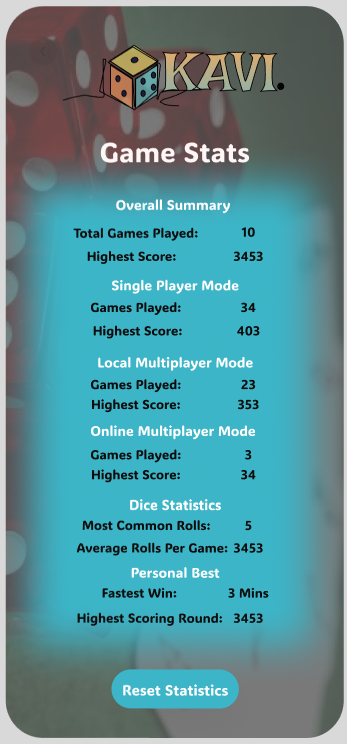
\includegraphics[scale=0.45]{img/stats.png}
        \caption{Design page 2}
        \label{fig:figma_design2}
    \end{subfigure}
    \caption{Initial UI designs and prototypes created in Figma}
    \label{fig:figma_designs}
\end{figure}

\subsection{Design Process}
The application's design process began with creating detailed wireframes and prototypes in Figma. The designs underwent several iterations based on user feedback and technical constraints, evolving into the final implementation. Figure~\ref{fig:figma_designs} shows some of the initial design concepts and their evolution \cite{bib:kavifigma}.

Various existing solutions and design tools inspired the design of the application, one of which stood out was the board screen design was inspired by a dice application project by binaryshrey \cite{bib:binaryshrey}. This repository provided a minimalistic and intuitive approach to dice roll applications, which influenced the layout and functionality of the board screen in this project.

\subsection{Model Training}

The dice detection model was developed using Roboflow's platform, which streamlined the entire process from dataset creation to deployment. The training dataset, depicted in Figure~\ref{fig:roboflow_dataset}, consisted of carefully annotated dice images across various conditions, ensuring robust detection performance in real-world scenarios.

\begin{figure}[h]
    \centering
    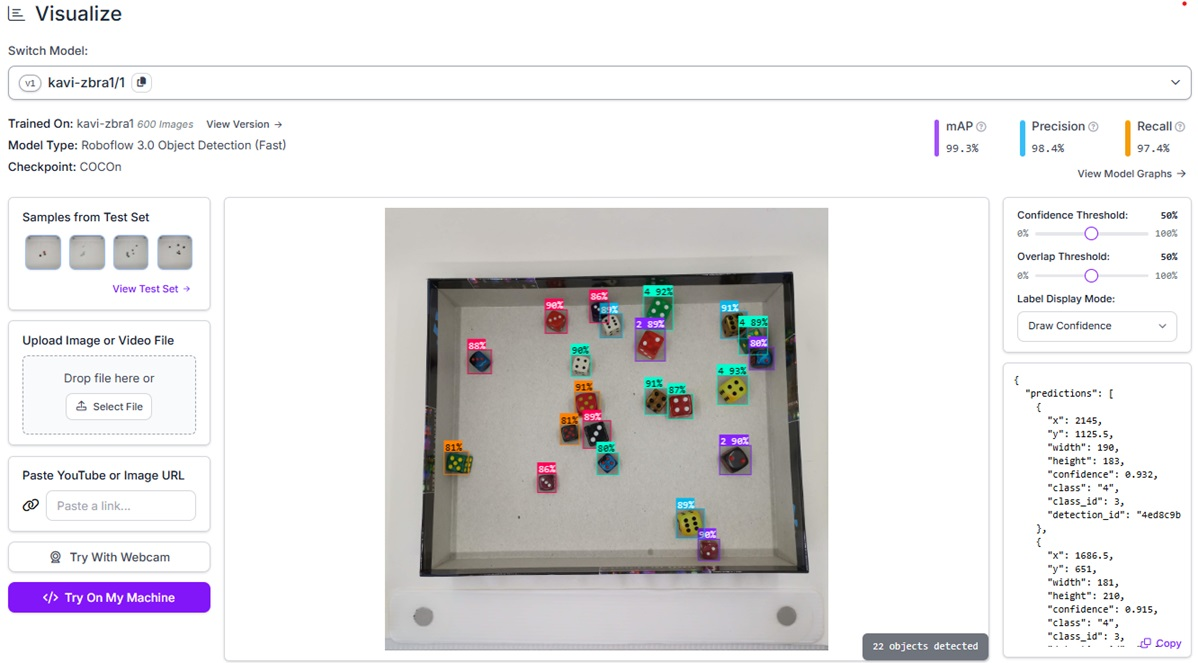
\includegraphics[width=\textwidth]{img/roboflow_dataset.jpg}
    \caption{Roboflow dataset management interface showing dice image annotations}
    \label{fig:roboflow_dataset}
\end{figure}

Roboflow facilitated data augmentation and preprocessing, which enhanced the dataset's diversity. The model training and optimization phases were crucial for achieving high accuracy, while the deployment and API integration ensured seamless real-time inference capabilities.

\subsection{Project Timeline}

The project was implemented from November 2024 to January 2025, following a structured timeline as shown in Figure~\ref{fig:gantt}. The development process was organized into major phases, including planning, design, core development, AI integration, and testing, with regular milestones to track progress.

\begin{figure}[h]
    \centering
    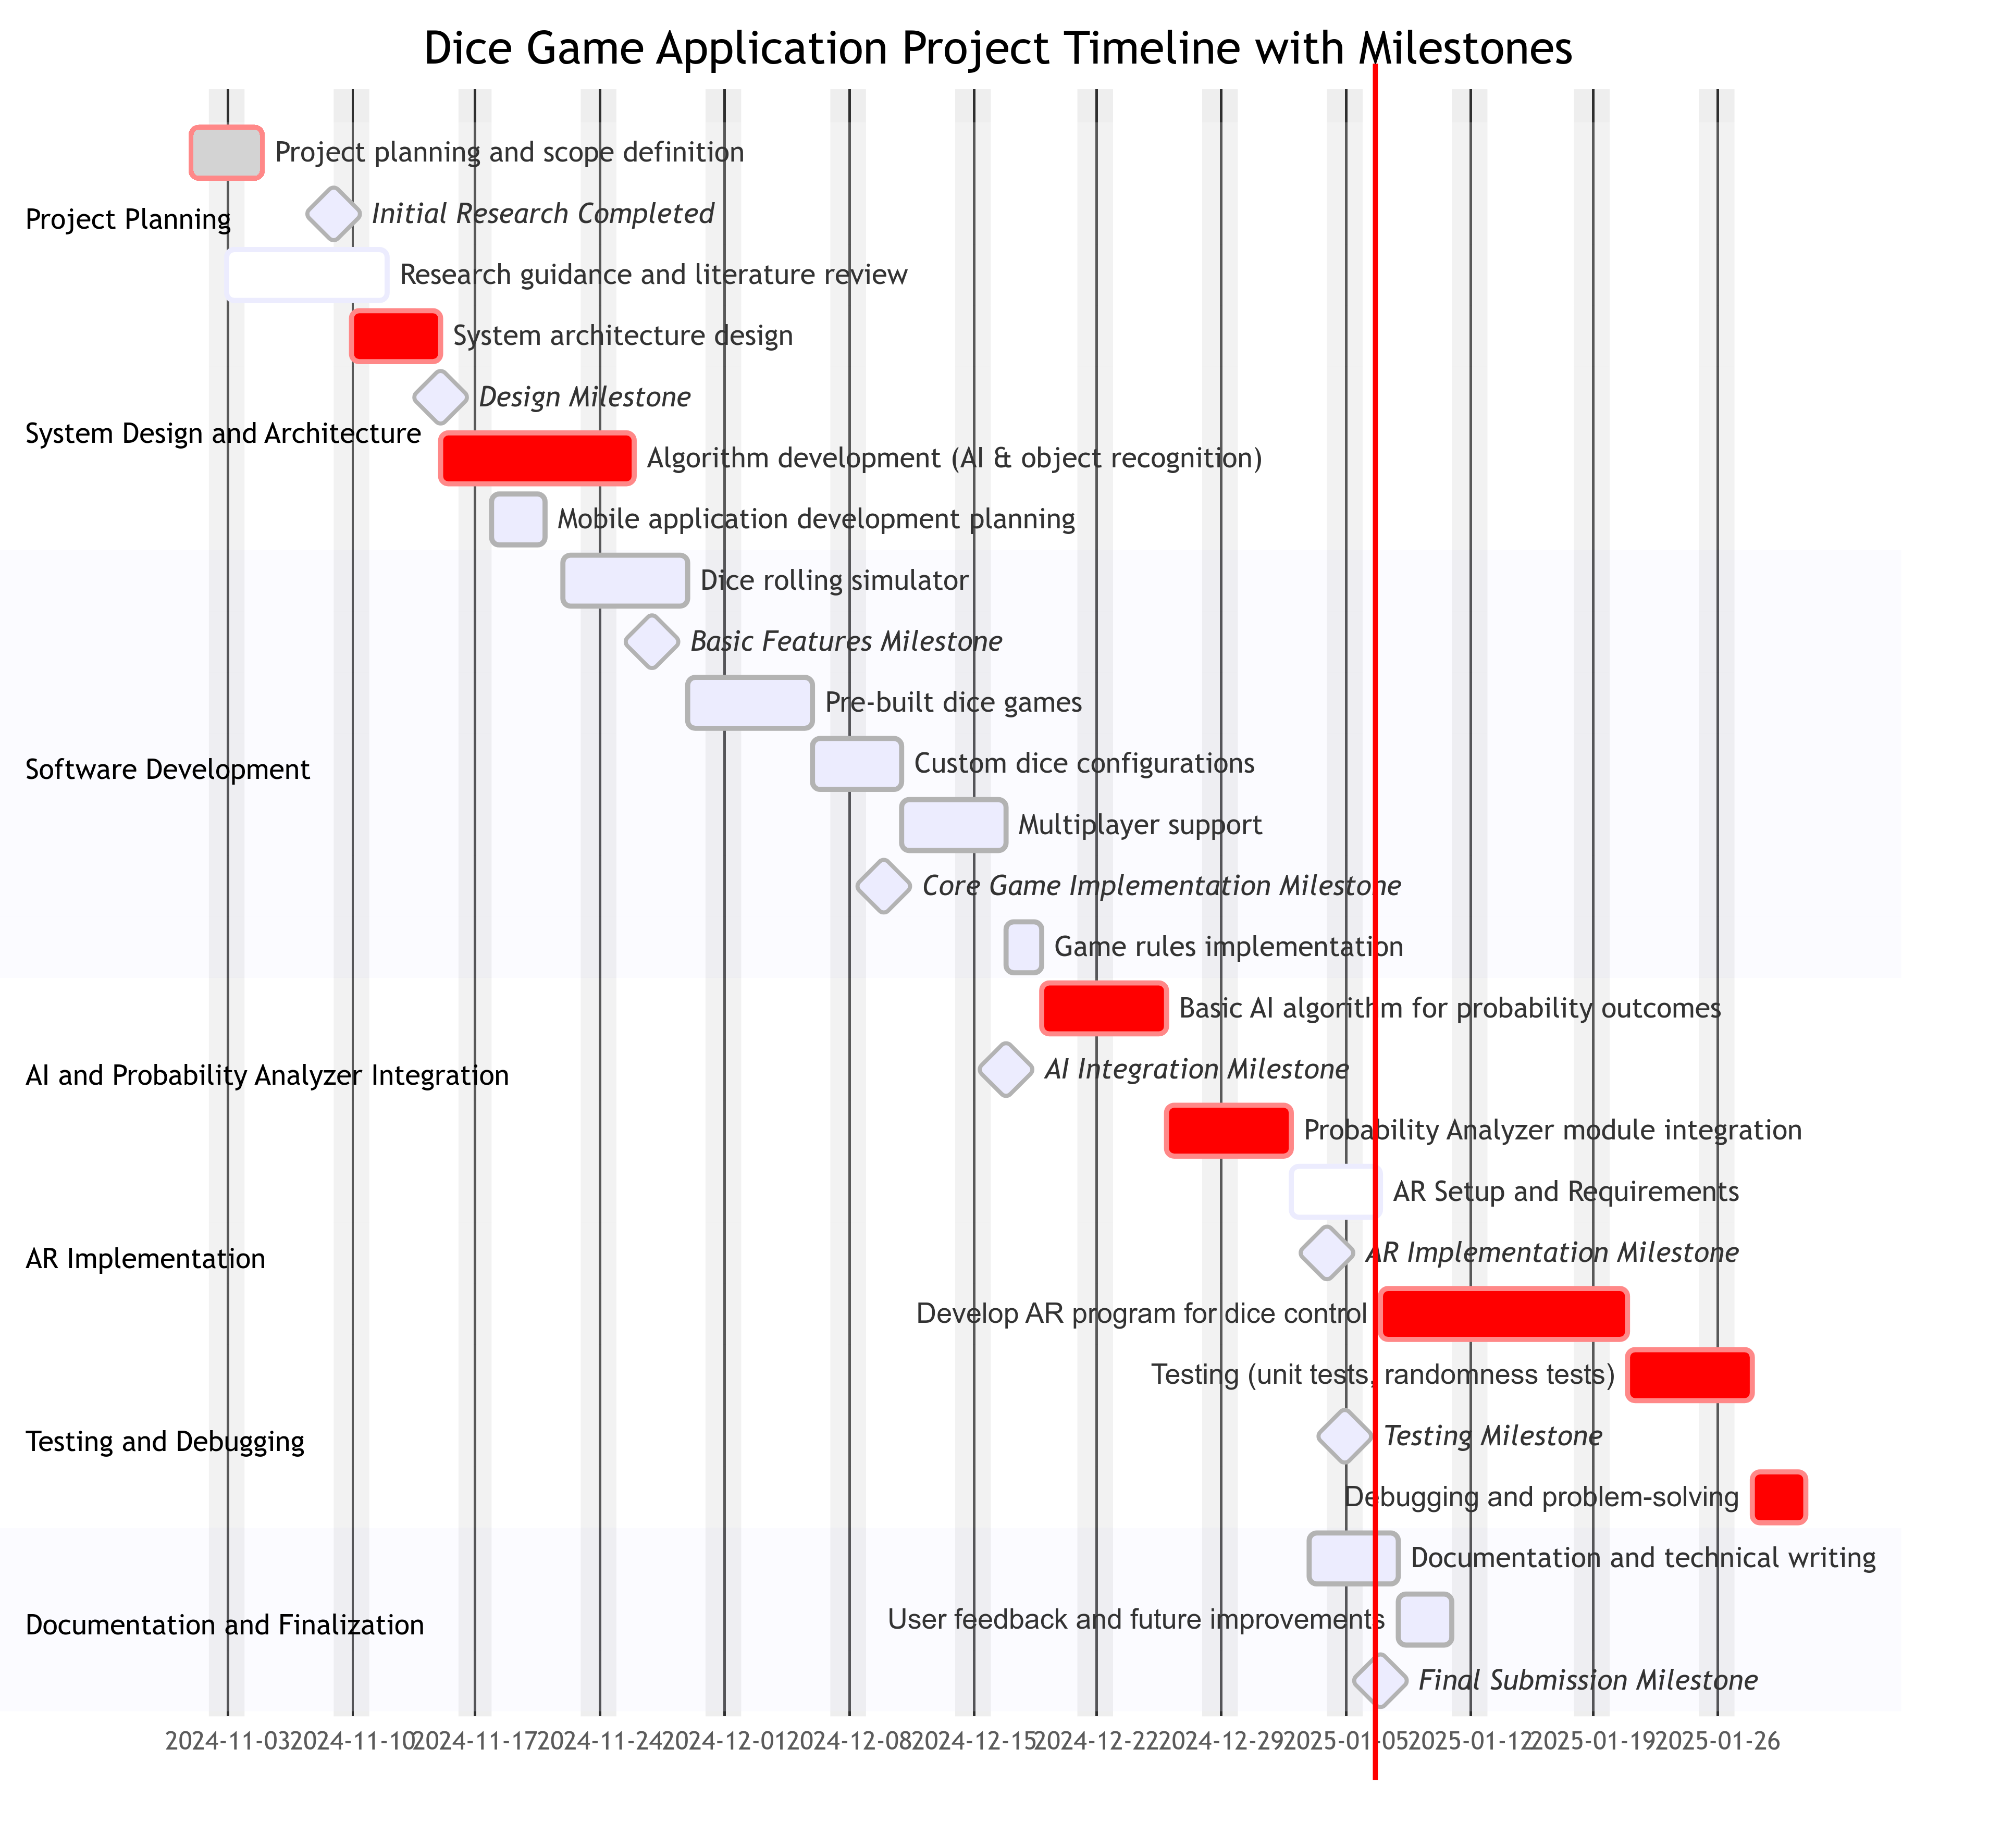
\includegraphics[width=\textwidth]{img/gantt_chart.png}
    \caption{Project Gantt chart showing development phases and milestones}
    \label{fig:gantt}
\end{figure}

This structured approach allowed for continuous improvement and adaptation to changing requirements, ensuring a high-quality application. While some initially planned features like AR implementation were identified as future enhancements, the focus remained on delivering a robust core game experience with AI capabilities.